\chapter{MATERIALS AND METHODS}

\section{Consensus \emph{S. cerevisiae} Metabolic Model}
Variety of \emph{S. cerevisiae} genome-scale metabolic models have been used since 2003, and each reconstructed model introduced more manual curations, increasing gene numbers from annotations and better predictions regarding the previous ones \cite{lopes2017genome}. A consensus genome-scale metabolic model of \emph{S. cerevisiae}, Yeast8, is presented in an open-source, version-controlled maintainable way in 2019, claiming that the model can be represented and investigated in a systematic way using Git (https://git-scm.com/) and GitHub (https://github.com/) as a hosting service for the model repository \cite{lu2019consensus}. Systematic way of Yeast8 enables to study simultaneously in collaborative studies, provides record keeping of model changes, version updates, where each version of can be released periodically and accessible all the time (Figure \ref{fig:yeast8_github}).

Yeast8 model can be considered as an updated version of Yeast7 \cite{aung2013revising} with additional corrections based on the annotations available in KEGG and ChEBI, and several gene inclusions from the model iSce926 \cite{chowdhury2015using}. Final version of Yeast8 to date, version 8.3.4 released on July 28, has 3991 reactions, 2691 metabolites, 1149 genes and 14 intracellular compartments. Additional statistical analysis on its stoichiometric matrix can be seen in Figure \ref{fig:modelstats}.

All simulations in the Methods section are done on the model Yeast8 v8.3.4 which is hosted in Github (https://github.com/SysBioChalmers/yeast-GEM). All optimization problems were solved with the COBRA Toolbox v3.0.6 in MATLAB (version 9.7.0.1216025 (R2019b)), using Gurobi solver (version 8.1.1).

\begin{figure}[H]
\begin{center}
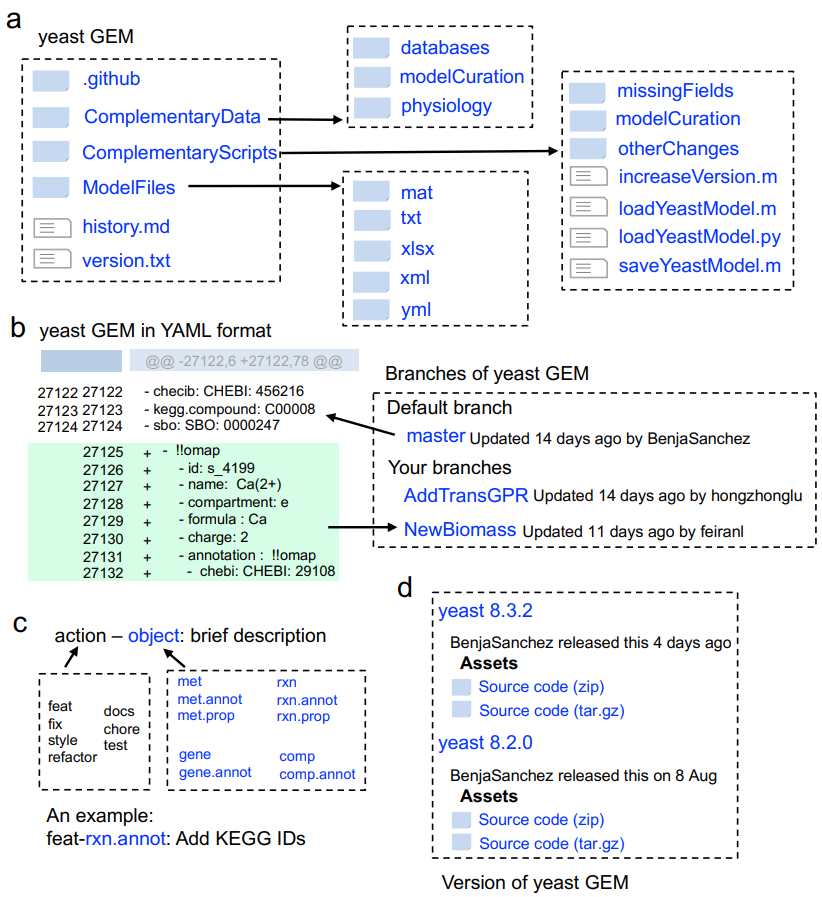
\includegraphics[width=1\columnwidth]{yeast8_github.png}
\end{center}
\caption[Repository of yeast GEM on GitHub]{Repository of yeast GEM on GitHub. Figure is taken from \cite{lu2019consensus}. ~ will be redrawned in the final version of the thesis.}
\label{fig:yeast8_github}
\end{figure}

\begin{figure}[H]
\begin{center}
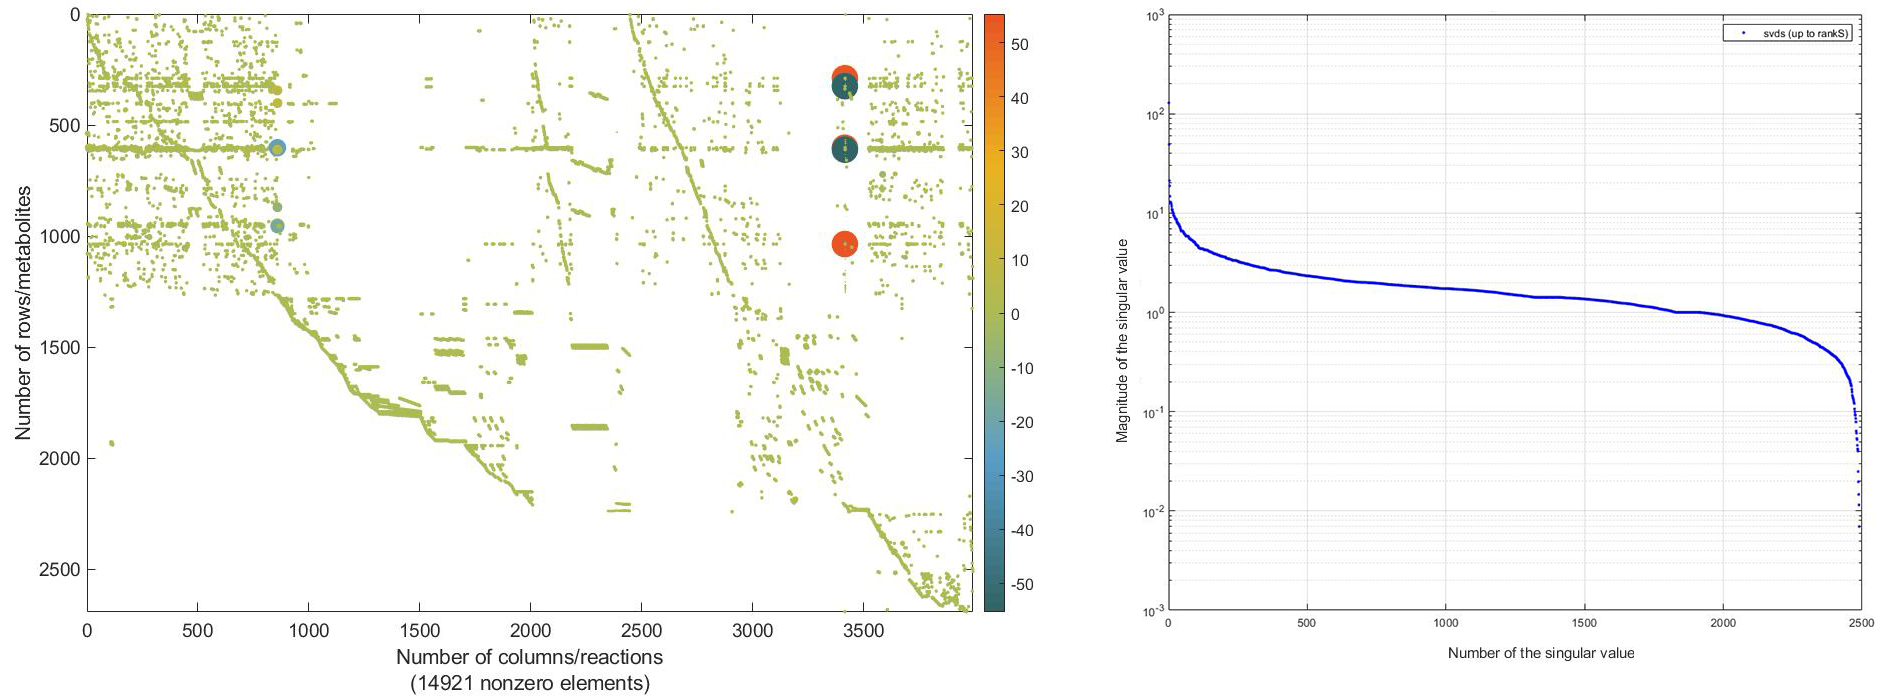
\includegraphics[width=1\columnwidth]{modelstats.png}
\end{center}
\caption[Coefficients and singular values of the stoichiometric matrix of Yeast8]{Coefficients and singular values of the stoichiometric matrix of Yeast8}
\label{fig:modelstats}
\end{figure}



\section{Flux Balance Analysis}
Flux balance analysis (FBA) assumes that the living cells act as they optimized their lives towards some goal, and as if they were at steady state. To be more clear, steady-state assumption indicates that the metabolites are both produced and consumed at the same rate in a cell, without an accumulation. Therefore, in this system, metabolites are constrained by only the stoichiometric coefficients arised from mass balance of metabolites. FBA solves a set of ordinary differential equations regarding to the stoichiometric matrix:
\begin{equation}
 \ S_{m \times n} \cdot v=0
\end{equation}
\noindent where S is the matrix of the stoichiometric reaction coefficients with m number of metabolites (as rows) and n number of reactions (as columns), and v is the vector of all associated reaction fluxes (mmol/gDWh). Because the matrix S usually has more reactions than metabolites (m<n), the system can result multiple solutions, and being called an underdetermined system (read more on Section \ref{metabolicnetworks}). To solve it for an optimal solution, additional constraints or an objective function is required.

A "growth reaction" is usually included in the reactions of the system to represent the "goal" in the definition of living systems. Growth reactions act as the final consumption of metabolites necessary for the biomass production or cell replication. Additional to the growth, several exchange reactions (uptake or secretion of metabolites from or into extracellular space) are also included. Since the concentrations of extracellular metabolites are measurable experimental, constraints can be applied to exchange reaction fluxes to shrink solution space. The more constraints introduced into the system, such as reversibility of reactions or known rate values, result smaller solution space. The growth reaction is usually used as an objective function to determine a unique solution from this solution space. The linear problem appears as:
\begin{align}
 \ \text{max}_v \quad & c^T \cdot v \\
 \label{eq:fba}
 \ \text{subject to} \quad & S_{m \times n} \cdot v=0 \\
 \ & v_{lb} \leq v \leq v_{ub}
\end{align}
\noindent where c is the objective function vector, v is the vector of fluxes, S is the stoichiometric matrix as in above equation. Subscripts lb and ub are the lower and upper boundaries on v. These constraints defines a feasible region of the problem. Coefficients of the biomass constituents are defined as the same as the batch conditions in the reference article \cite{nilsson2016metabolic}, for the reason that detailed knowledge is not available in the acquired experimental data (see section \ref{experimentaldataacquisition}). Coefficients for the final biomass equation can be found in the Table \ref{table:biomass_coefficients}.

\begin{table}[H]
\vskip\baselineskip
\caption[Biomass coefficients]{Biomass coefficients that are used in the FBA simulation (numbers are not updated)}
\begin{center}
  \begin{tabular}{ll}
  \hline
  \textbf{Constituent} & \textbf{Coefficient} \\ \hline
  Protein              & 3.703704             \\
  RNA                  & 0.37037              \\
  DNA                  & 0.018519             \\
  Lipid                & 0.041667             \\
  Glycogen             & 0.030864             \\
  Trehalose            & 0.029214             \\
  Mannan               & 0                    \\
  Glucan               & 2.469136             \\
  Maintainance         & 40                   \\ \hline
  \end{tabular}
\label{table:biomass_coefficients}
\end{center}
\end{table}



\section{Experimental Data Acquisition} \label{experimentaldataacquisition}
Extracellular metabolomics data are obtained from Cakar's Lab \cite{arslan2018physiological}. Briefly, they perform ethyl methane sulfonate (EMS) mutagenesis  on the prototrophic \emph{Saccharomyces cerevisiae} strain CEN.PK 113-7D (MATa, MAL2-8c, SUC2) to increase the genetic diversity as an evolutionary engineering selection strategy. Cells were inoculated in 2\% Yeast Minimal Media (YMM), and the extracellular concentrations of glucose, ethanol, glycerol and acetate were measured at different time points. OD\textsubscript{600} values were determined by a spectrophotometer. Additionally, cell dry weight analysis was conducted to determine biomass production. Acquired extracellular metabolite concentrations, OD\textsubscript{600} values and dry weights of the reference strain (without mutagenesis) were used in this study are collected in Table \ref{table:experimental_data} and Table \ref{table:experimental_OD600s_and_growths}.

\begin{table}[H]
\caption[Measured OD\textsubscript{600} and cell dry weight values of reference strain \cite{surmeli2019evolutionary}]{Measured OD\textsubscript{600} and cell dry weight values of reference strain \cite{surmeli2019evolutionary}.}
\begin{center}
  \begin{tabular}{|c|c|c|c|}
 \hline
  \textbf{Time (h)} & \textbf{OD600} & \textbf{ln(OD600)} & \textbf{Cell DW (g/L)} \\
  \hline
  0                 & 0.21           & -1.560647748       & -                      \\
  3                 & 0.53           & -0.634878272       & -                      \\
  6                 & 1.76           & 0.565313809        & 0.9                    \\
  7.5               & 2.66           & 0.978326123        & -                      \\
  9                 & 4.46           & 1.495148766        & 1.9                    \\
  12                & 5.31           & 1.669591835        & -                      \\
  15                & 5.88           & 1.771556762        & -                      \\
  18                & 5.83           & 1.763017           & 2.32                   \\
  21                & 6.07           & 1.803358605        & -                      \\
  24                & 5.87           & 1.769854634        & -                      \\
  30                & 6.14           & 1.814824742        & 2.26                   \\
  40                & 6.44           & 1.86252854         & -                      \\
  46                & 6.36           & 1.850028377        & -                      \\
  50                & 6.3            & 1.840549633        & -                      \\
  54                & 6.55           & 1.87946505         & -                      \\
  63                & 6.54           & 1.877937165        & -                      \\
  67                & 6.88           & 1.928618652        & -                      \\
  72                & 6.97           & 1.941615225        & 2.66                  \\
   \hline
  \end{tabular}
\label{table:experimental_OD600s_and_growths}
\end{center}
\end{table}

\begin{table}[H]
\caption[Measurements of extracellular concentrations \cite{surmeli2019evolutionary}]{Measurements of extracellular concentrations \cite{surmeli2019evolutionary}.}
\begin{center}
\begin{tabular}{|c|c|c|c|c|}
   \hline
  \textbf{Time(h)} & \textbf{Glucose(g/L)} & \textbf{Ethanol(g/L)} & \textbf{Glycerol(g/L)} & \textbf{Acetate(g/L)} \\
    \hline
  0                 & 19.99            & 0                & 0                 & 1.08             \\
  3                 & 17.98            & 0.58             & 0.02              & 1.24             \\
  6                 & 15.85            & 1.2              & 0.06              & 1.16             \\
  9                 & 12.21            & 3.39             & 0.18              & 1.37             \\
  12                & 9.18             & 7.97             & 0.61              & 2.45             \\
  15                & 0.4              & 8.17             & 0.69              & 2.46             \\
  27                & 0                & 8.28             & 0.76              & 2.6              \\
  46                & 0                & 8                & 0.77              & 2.45             \\
  50                & 0                & 6.62             & 0.64              & 2.02             \\
  54                & 0                & 5.74             & 0.55              & 1.73             \\
  58                & 0                & 5.46             & 0.54              & 1.74             \\
  72                & 0                & 3.72             & 0.49              & 1.33            \\
   \hline
\end{tabular}
\label{table:experimental_data}
\end{center}
\end{table}


As the slope in the curve of lnOD\textsubscript{600} as a function of time gives the growth rates of cells, natural logarithm of OD\textsubscript{600} values were calculated to obtain specific growth rates by using the equation \ref{eq:growthrates}.
  \begin{equation}
      \ \mu = \frac{\Delta \ln{OD_{600}}}{\Delta t}
      \label{eq:growthrates}
  \end{equation}

In order to determine uptake and secretion rates of the metabolites, the steady-state assumption is applied in three hours intervals as the shortest measured time-points. Missing data on cell dry weights are estimated from the OD\textsubscript{600} values, and these cell dry weight data is used to calculate fluxes (in the unit of mmol/gDWh). Measurement of the cell dry weight at the 3rd hour was crucial for the steady-state assumption, however data was not available from the experiments. Curve trend of the OD\textsubscript{600} plot is used as a guide to estimate cell dry weight (Figure \ref{fig:GrowthGraphs}).
\begin{figure}[H]
  \begin{center}
  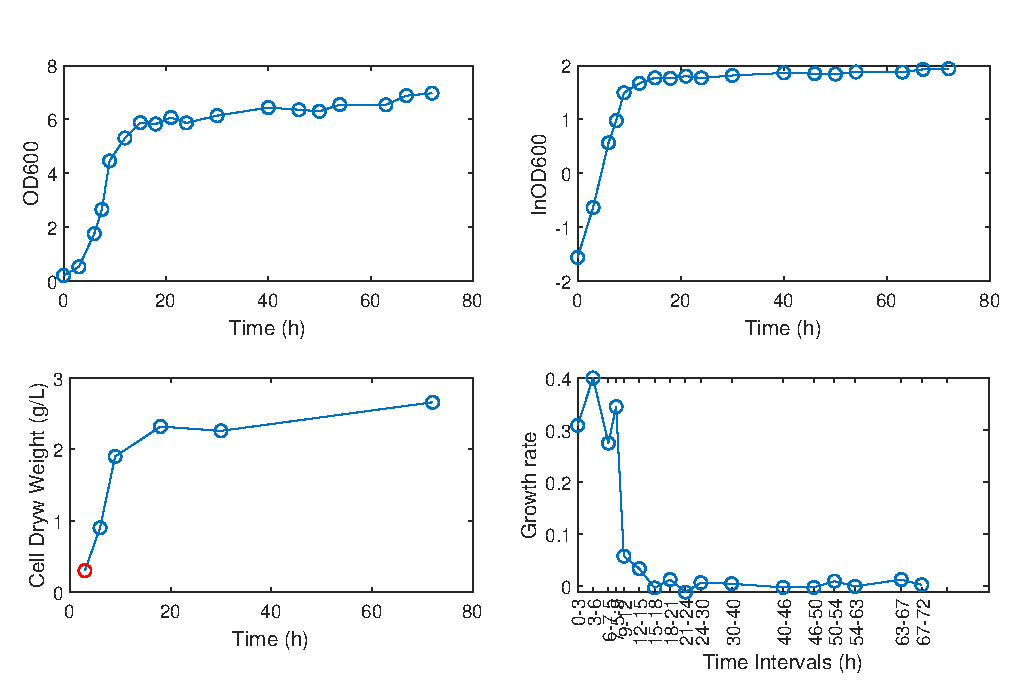
\includegraphics[width=1\columnwidth]{GrowthGraphsSmall.eps}
  \end{center}
  \caption[OD\textsubscript{600}, lnOD\textsubscript{600}, cell dry weights and growth rates]{OD\textsubscript{600}, lnOD\textsubscript{600}, cell dry weights and growth rates graphs. Estimated missing cell dry weight data is shown in red color.}
\label{fig:GrowthGraphs}
\end{figure}



\section{Batch Simulation}
In order to simulate batch conditions where minimal yeast medium is used, all the exchange reactions in the model are blocked first (lower bounds are set to 0). Then, only the exchange reactions of ions that are available to the cells in the experimental design (ammonium, phosphate, sulphate, iron(2+), H+, water, chloride, Mn\textsuperscript{2+}, Zn\textsuperscript{2+}, Mg\textsuperscript{2+}, sodium, Cu2\textsuperscript{2+}, Ca\textsuperscript{2+}, potassium) are set free (lower bounds are set to -1000), means that cells can uptake as it needs. While oxygen and glucose uptake rates decreased from 20 mmol gDWh\textsuperscript{-1} and increased to 20 mmol gDWh\textsuperscript{-1}, respectively, fluxes of ethanol, acetate, glycerol, formate, succinate secretion reactions with the growth rate is collected.


\section{Integration of Enzymatic Constraints}

Solution space of the Yeast8 can be further constrained by limiting fluxes of reactions with integration of enzymatic informations by using GECKO (GEM with Enzymatic Constraints using Kinetic and Omics data) method \cite{sanchez2017improving}.  In GECKO methodology, if a reaction has an annotated enzyme requirement in order to occur in the cell, extra enzyme entity is included in the reaction equation itself. Stoichiometric coefficient of this entity is defined by its kinetic information and abundance in the cell (Figure \ref{fig:gecko1}). S matrix of the system is expanded with the addition of new rows for the enzymes and new columns for the each enzyme's usage.

\begin{figure}[H]
\begin{center}
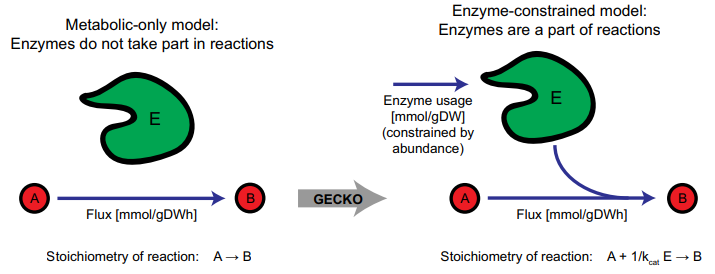
\includegraphics[width=1\columnwidth]{gecko1.png}
\begin{align}
\label{eq:geckoreaction}
 \ A \xrightarrow{E_i} B \\
 \label{eq:gecko}
 \ A + n_{ij}E_i \xrightarrow{} B
\end{align}
\end{center}
\caption[GECKO]{GECKO, will be redrawn.}
\label{fig:gecko1}
\end{figure}

The idea behind this methodology arises from the biochemical constraints, such that the maximum rate of a reaction is smaller or equal to its enzyme's turnover number and the concentration (mmol/gDW).
\begin{align}
 \label{eq:gecko_simple}
 \ v_{j} \leq k_{cat}^{ij} \cdot [E_{i}]
\end{align}
Enzymes in the reaction equations must be considered as pseudo-metabolites because they do not affect the mass balance of the reaction, i.e. enzymes are not consumed in the reactions but they are occupied for a short period of time. To maintain mass balances of enzymes, an overall enzyme usage pseudo-reaction is introduced into system in order to supplement enzymes into rections, similar to exchange reactions:
\begin{align}
 \label{eq:gecko_suppelement}
 \  EU_i: \quad \to E_i
 \
\end{align}
If the flux carried by this reaction is $e_i$, we can say that $e_i$ ranges from 0 (i.e. no enzyme available) to a maximum value of $[E_i]$ (i.e. all the enzyme is used in the reaction):
\begin{align}
 \label{eq:gecko_enzymeflux}
 \  0 \leq e_i \leq [E_i]
\end{align}
Then a mass balance for the enzyme $E_i$ can be defined under steady state assumption:
\begin{align}
 \label{eq:gecko_enzymemass}
 \  -n_{ij} \cdot v_j + e_i = 0
\end{align}
By rearranging the equations \ref{eq:gecko_enzymeflux} and \ref{eq:gecko_enzymemass}, we obtain:
\begin{align}
 \label{eq:gecko_enzymemassrearranged}
 \ v_j \leq \frac{1}{n_{ij}} \cdot [E_i]
\end{align}
and if we compare this equation with the equation \ref{eq:gecko_simple}, we can finally calculate the stoichiometric coefficient for the enzyme.
\begin{align}
 \label{eq:gecko_enzymestoichiometry}
 \ n_{ij}=\frac{1}{k_{cat}^{ij}}
\end{align}

However the equation \ref{eq:gecko_simple} does not hold in all cases since reactions can be more complex. For isozymes in which multiple enzymes catalyze the same reaction, the equation becomes:
\begin{align}
 \label{eq:gecko_isozymes}
 \ v_{j} \leq \sum\limits_{i} k_{cat}^{ij} \cdot [E_{i}]
 \
\end{align}
Since the reaction can be catalyzed by all the isozymes equally, new reactions can be defined for each isozyme (note that each enzyme can have different $k_{cat}$ values). For example, if we think that the equation \ref{eq:geckoreaction} had two isozymes, $A \xrightarrow{E_1 or E_2} B$, the new reactions defined would be,
\begin{align}
 \ R_{j/1}: \quad \frac{1}{k_{cat}^{1j}}E_1 + A \to B \\
 \ R_{j/2}: \quad \frac{1}{k_{cat}^{2j}}E_2 + A \to B
\end{align}
These additional reactions distrupt the boundaries for the initial reaction. In order to maintain original boundaries, another "arm-reaction" is also introduced to the system where it acts as an intermediate metabolite.
\begin{align}
 \ R_{j/arm}: \quad A \to M_{int} \\
 \ R_{j/1}: \quad \frac{1}{k_{cat}^{1j}}E_1 + M_{int} \to B \\
 \ R_{j/2}: \quad \frac{1}{k_{cat}^{2j}}E_2 + M_{int} \to B
\end{align}

%For an enzyme that can catalyze multiple reactions,the for each reaction:
%\begin{align}
% \label{eq:gecko_promiscuous}
% \ \sum\limits_{j} \frac{ v_{j} }{ k_{cat}^{ij} } \leq [E_{i}]
% \
%\end{align}

For an enzyme complex catalyzing a single reaction, since the reaction is catalyzed by all the enzymes which share the same $k_{cat}$ value, the equation \ref{eq:gecko_simple} becomes:
\begin{align}
 \label{eq:gecko_complex}
 \ v_{j} \leq  k_{cat}^{ij} \cdot \min\limits_{k} \frac{ [U_{ik}] }{ S_{ik} }
 \
\end{align}
\noindent where $[U_{ik}]$  is the concentration of the subunit of the catalyzing enzyme $E_{i}$, and $S_{ik}$ is the stoichiometry of the subunit. For the reaction, if we think that the equation \ref{eq:geckoreaction} was catalyzed by an enzyme complex of 2 subunits, $A \xrightarrow{E_1 and E_2} B$, then it would be:
\begin{align}
 \label{eq:gecko_complex2}
 \ R_{j}: \quad \frac{S_1}{k_{cat}^{ij}}E_1 +\frac{S_2}{k_{cat}^{ij}}E_2 + A \to B
\end{align}

Finally, for the reversible reactions, two reactions must be defined for both forward and backward direction reactions with the same catalyzing enzyme but possibly with different $k_{cat}$ values. Assume the equation \ref{eq:geckoreaction} is reversible, following equations would be introduced to the system:
\begin{align}
 \label{eq:gecko_reversible}
 \ R_{j/f}: \quad \frac{1}{k_{cat}^{ij/f}}E_i + A \to B \\
 \ R_{j/b}: \quad \frac{1}{k_{cat}^{ij/b}}E_i + B \to A
\end{align}



\section{Integration of Transcriptome Data}
Transcriptome data is initially converted into protein abundances and used to change the stoichiometry of the enzyme usage pseudo-reaction. Will be explained when a solid function for expression=abundance assumption is found.


\section{Phenotype Phase Plane Construction}

As previously mentioned, there is no single solution to the linear problem of the model. Phenotype phase planes (PhPP) are used to describe all feasible metabolic states in a two or three dimentional surfaces, depending on the number of metabolites chosen to see how they affect the objective function \cite{edwards2002characterizing}. In general, for aerobic models, various levels of glucose and oxygen availability through their uptake reactions are used to generate PhPP surfaces in three dimention with objective function. Fundamentally, PhPP construction refers to a double robustness analysis on the model for selected reactions.


\section{Flux Variability Analysis}
Flux variability analysis (FVA) finds the minimum and maximum available fluxes for each reaction while obeying the provided constraints (for example fixed glucose uptake or growth rate). FVA is mainly used to evaluate the robustness of the model \cite{thiele2010functional}, to find alternative optimum states \cite{mahadevan2003effects}, to check flux distributions when growth is not at optimum level \cite{reed2004genome}, and it has many other applications \cite{gudmundsson2010computationally}.

FVA, similar to FBA, solves two optimization problems for each reaction:
 \begin{align}
 \ \text{max}_v / \text{min}_v \quad & v_i \\
 \ \text{subject to} \quad & S_{m \times n} \cdot v=0 \\
 \ & w^T \cdot v \geq \gamma \cdot Z_0 \\
 \ & v_{lb} \leq v \leq v_{ub}
 \end{align}
\noindent where $w$ is the objective function equals to $c$ in the problem \ref{eq:fba}, $Z_0 = w^T \cdot v_0$ describes an optimal solution to the problem \ref{eq:fba}, $\gamma$ is an indicator to check whether the FVA is done at the optimal state (where objective flux is the same and $\gamma = 1$) or any other state (where $0 \leq \gamma < 1$).


\section{Random Sampling of Solution Space}
Constraints applied to a model define a solution space, a convex polytope, where every flux distribution is accessible. Random sampling of the solution space is an unbiased tool to explore metabolic models. Mainly, Markov Chain Monte Carlo methods are used to sample this space using algorithms such as (Artificially Centered) Hit-and-Run (HRB) \cite{kiatsupaibul2011analysis, saa2016ll} algorithm, and this method has proven to be helpful in the analysis of genome-scale metabolic models \cite{schellenberger2009use}. Briefly, the random sampling method collects points that are uniformly distributed in the solution space and calculates the most probable flux value for each reaction.

\begin{figure}[H]
\begin{center}
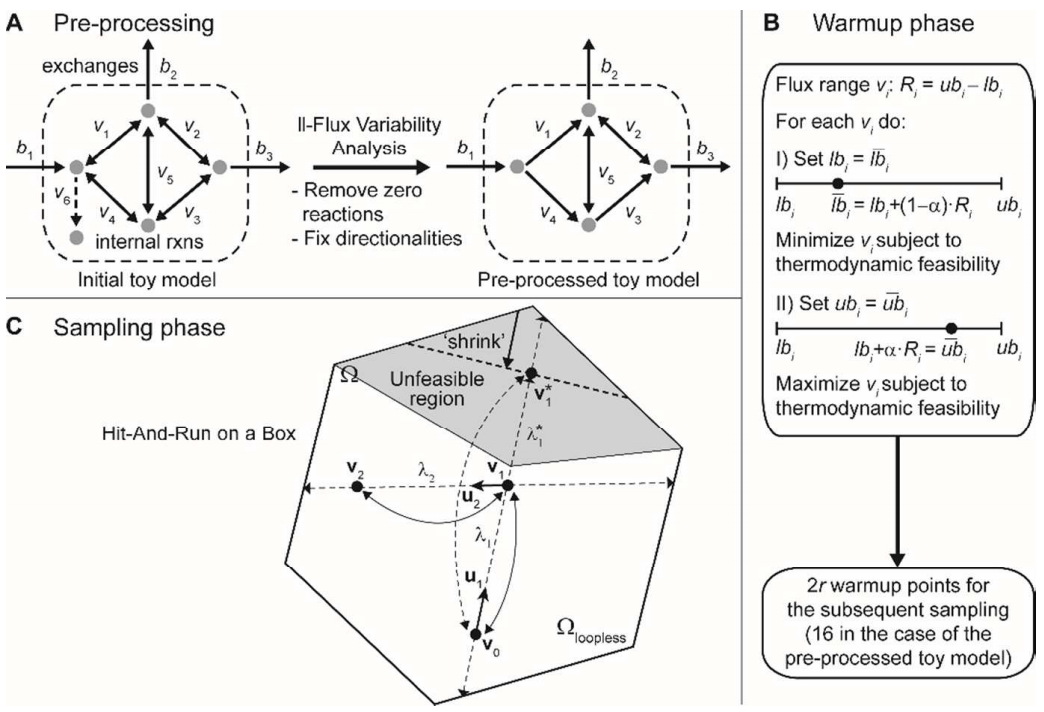
\includegraphics[width=1\columnwidth]{ll-achrb.png}
\end{center}
\caption[Workflow of the Loopless-ACHRB sampling on a toy model]{Workflow of the ll-ACHRB sampling on a toy model. A) Pre-processing phase, application of loopless-FBA to remove blocked reactions and constraining the directionalities of others. B) Warmup phase, modifying the reaction bounds to more interior space. C) Sampling phase with HRB algorithm. Figure is taken from \cite{saa2016ll}}
\label{fig:achrb}
\end{figure}

Since the computational burden of loopless sampling is high, generated random points in the solution space of Yeast8 includes thermodynamically unfeasble states. Maximum glucose uptake rate was constrained to 1 mmol gDWh\textsuperscript{-1} and total of 5000 points are generated with maximum of 120 secondse alloted for the sampling.
